\documentclass[12pt]{article}
\usepackage{amsfonts}
\usepackage{graphicx}
\usepackage[utf8x]{inputenc}
\usepackage{amsmath}
\usepackage{graphicx}
\usepackage[colorinlistoftodos]{todonotes}
\usepackage{float}

%%%%%%%%%%%%%%%%%%%%%%%%%%%%%%%%%%%%%%%%%%%%%%%%%%%%%%%%%%%%%%%%
%
% dimensions choisies par l'utilisateur (bricolage personnel)

\newdimen\decalage

\paperheight=29.7 true cm \paperwidth=21 true cm
\textheight=22.7 true cm \textwidth=17 true cm
\decalage=0 true cm

% déduction de \topmargin,
% \evensidemargin et \oddsidemargin

\oddsidemargin=\paperwidth
\advance\oddsidemargin by -\textwidth
\divide\oddsidemargin by 2
\advance\oddsidemargin by -1 in
\evensidemargin=\oddsidemargin
\advance\oddsidemargin by \decalage 
\advance\evensidemargin by -\decalage

\topmargin=\paperheight
\advance\topmargin by -\headheight
\advance\topmargin by -\headsep
\advance\topmargin by -\textheight
\advance\topmargin by -\footskip
\divide\topmargin by 2
\advance\topmargin by -1 in

%
%%%%%%%%%%%%%%%%%%%%%%%%%%%%%%%%%%%%%%%%%%%%%%%%%%%%%%%%%%%%%%%%

\begin{document}
\title{Simulation Serveur Web}
\author{Jean-Marc Celesti \\ Yohann Hako Moukam}
\date{30 Novembre 2015}
\maketitle


\section{Exercice 1}
\subsection{Question 1}
\textit{Justifier pourquoi le temps moyen de réponse est d'au moins 49ms, indépendamment de $\lambda$. \\}

Soit $X$ la variable aléatoire qui estime le temps de réponse d'un utilisateur. On peut donc écrire $X$ = $X_{1}$ + $X_{2}$ avec :\\
- $X_{1}$ le temps d'attente avant que la requête soit traitée par le serveur (dépendant de $\lambda$).\\
- $X_{2}$ le temps de traitement de la requête (type 1 et 2) par le serveur.\\
Ce qui nous donne :\\
\[ E[X] = E[X_{1}] + E[X_{2}] = f(\lambda) + E[X_{2}] \]

avec : 
\[ E[X_{2}] = 2*RTT + E[R_{1}] + E[R_{2}]\]

\noindent - $R_{1}$ suit une loi uniforme sur (0 ; 30) : $E[R_{1}]$ = 15 \\
- $R_{2}$ suit une loi exponentielle de paramètre $\lambda$ = 0.1 . On a donc $E[R_{2}]$ = $\frac{1}{\lambda}$ = 10

d'ou :
\[ E[X_{2}] = 2*24 + 15 + 10 = 49\]

Par conséquent :
\[ E[X] = E[X_{1}] + 49 = f(\lambda) + 49 \geq 49 \]

\subsection{Question 2}
\textit{Programmer un simulateur à évènement discret et le décrire brièvement dans votre compte rendu \\}

Le principe du simulateur est le suivant : Tout d'abord une phase d'initialisation, où des dates d'arrivée sont générées via une loi exponentielle de paramètre $\lambda$ pour modéliser un processus de Poisson. Ces évènements (date d'arrivée,$R_{1}$) sont ensuite placés dans une file de priorité. \\

Les évènements $R_{1}$ sont décrits par la classe \textit{Type1}. Ils possèdent comme attribut principal la date de départ. Les évènements $R_{2}$ (classe \textit{Type2}) possèdent également une date de départ, en plus de conserver le temps écoulé depuis le début de la première requête qui l'a engendrée.\\

Le simulateur conserve une horloge qui est mise à jour après chaque évenement. Si au moment de retirer un évenement de la file, sa date théorique d'exécution est inférieure à celle de l'horloge (ce qui signifie donc que l'évènement est resté en attente avant d'être traité), on met à jour le temps d'attente de l'utilisateur. Au contraire, si la valeur de l'horloge est inférieure, on met à jour l'horloge (à la date d'execution de l'évènement) avec un temps d'attente nul.\\

Lorsqu'un évènement est retiré de la file, si il est de \textit{Type1}, on détermine le temps de la requête (sans oublier le RTT) et on ajoute à la file d'attente un évènement de \textit{Type2} avec en mémoire le temps écoulé. Si il est de \textit{Type2}, on calcule le temps de réponse de l'utilisateur.\\

Une liste des utilisateurs connectés est mise à jour à chaque itération. En effet, le simulateur regarde dans la file d'attente toutes les arrivées qui sont inférieures à la date actuelle. A la fin d'un évènement de \textit{Type2}, l'utilisateur est supprimé de la liste.\\

\subsection{Question 3}
\textit{Pour quelles valeurs de $\lambda$ [10 ; 100] requêtes/secondes le système vous semble stable ? \\} 

La valeur $\lambda$ = 30 semble être une valeur de lambda stable. En dessous, le système commence à saturer et le nombre d'utilisateurs en attente augmente de manière exponentielle. Les figures ci-dessous nous montrent la différence entre un système stable et un système instable.\\

\begin{figure}[H]
\centering
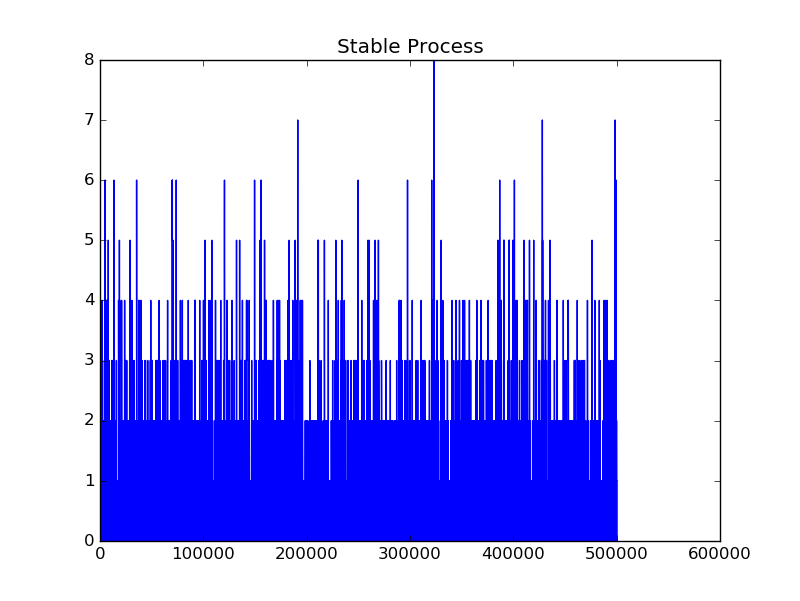
\includegraphics[scale=0.50]{stableprocessquestion3.png}
\caption{\label{fig:rf_taille_noeud} $\lambda$ = 100, $users$ = 5000}
\end{figure}

\begin{figure}[H]
\centering
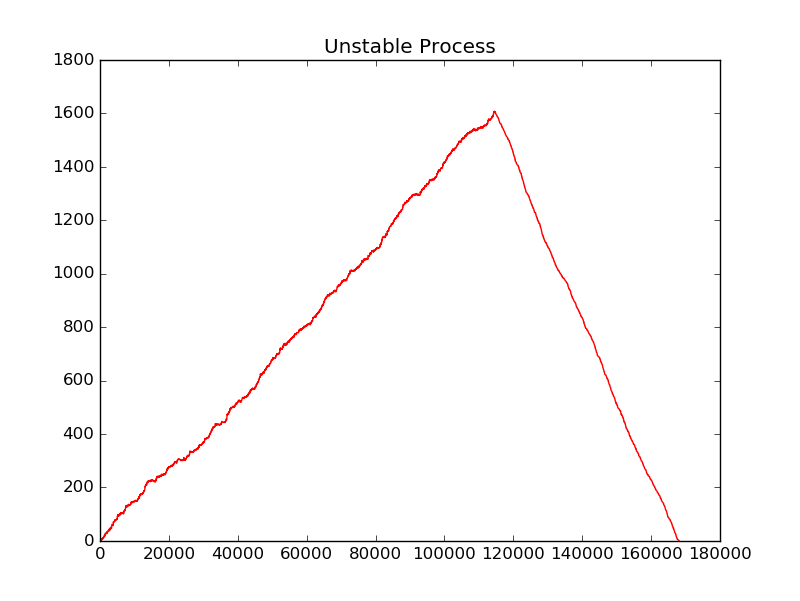
\includegraphics[scale=0.50]{unstableprocessquestion3.png}
\caption{\label{fig:rf_taille_noeud} $\lambda$ = 10, $users$ = 5000}
\end{figure}

La différence est logique et s'explique par le fait que moins il y a d'espacement entre les différentes arrivées (donc plus $\lambda$ est petit), plus l'utilisateur attend avant que sa requête ne soit traitée,car les arrivées s'enchâinent plus vite que le traitement des requêtes par le serveur. Le système commence à diverger. Lorsque $\lambda$ est grand ($\leq$ 20), les arrivées sont plus éloignées dans le temps et le serveur a le temps d'éxecuter les requêtes des utilisateurs sans trop attendre. 

\subsection{Question 4}
\begin{figure}[H]
\centering
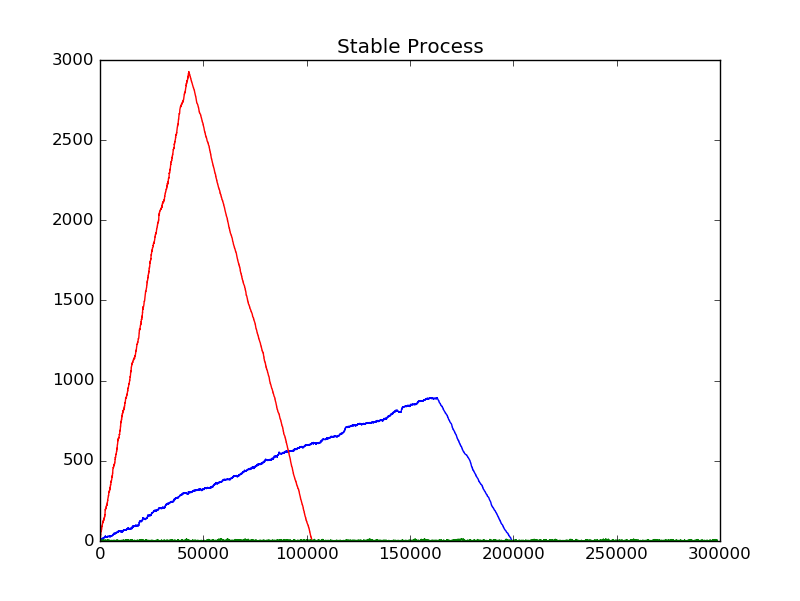
\includegraphics[scale=0.50]{3lambda.png}
\caption{\label{fig:rf_taille_noeud} $\lambda$ = 20,40,60, $users$ = 5000}
\end{figure}


\section{Exercice 2}
\subsection{Question 1}
\subsection{Question 2}
\textit{Reprendre les questions de l’exercice 1 avec la distribution de Pareto. Quelles différences observez vous ?}

\subsubsection{}
Le test avec une distribution de Pareto nous montre des résultats assez similaires pour les valeurs instables. En revanche, pour des valeurs supposées stables ($\lambda$ = 100), on observe un pic de connexions simultanées (totalement aléatoire). Les figures ci-dessous nous montrent les résultats obtenus avec Pareto.

\begin{figure}[H]
\centering
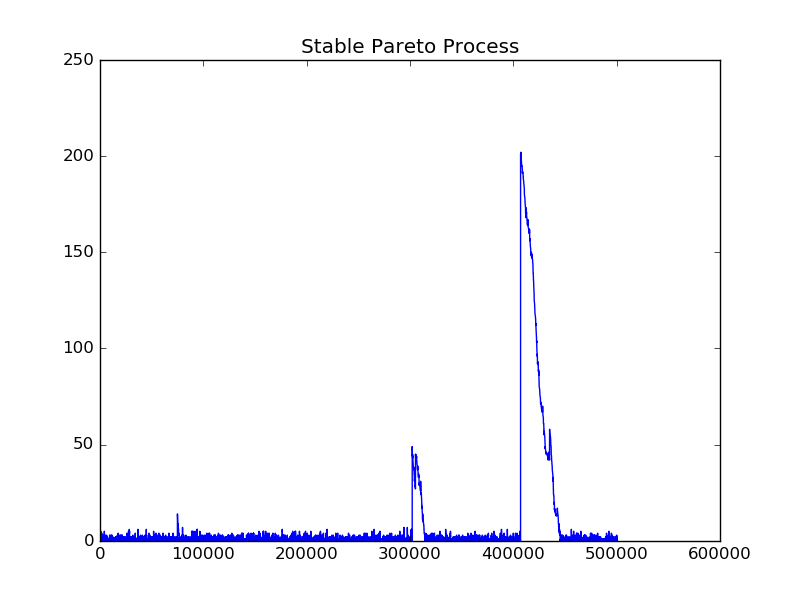
\includegraphics[scale=0.50]{stableprocessquestion3pareto.png}
\caption{\label{fig:rf_taille_noeud} $\lambda$ = 100, $users$ = 5000, Pareto}
\end{figure}

\begin{figure}[H]
\centering
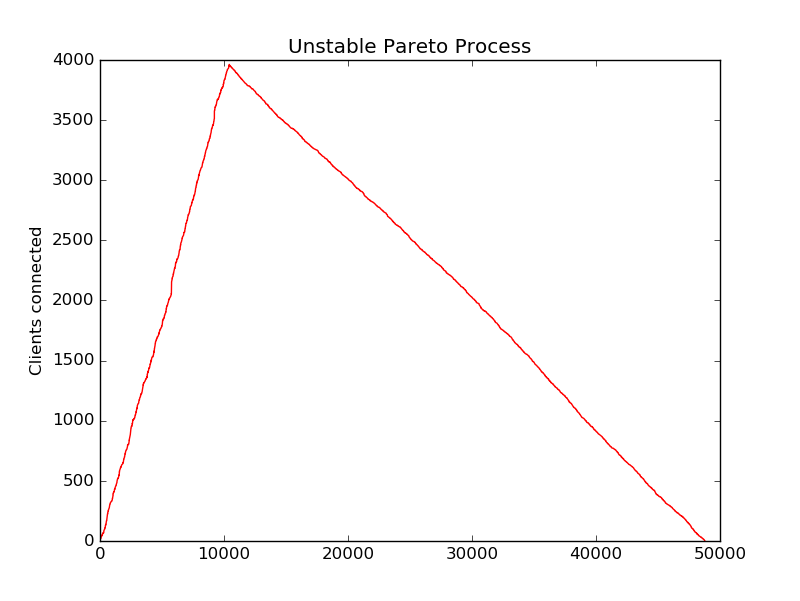
\includegraphics[scale=0.50]{unstablepareto.png}
\caption{\label{fig:rf_taille_noeud} $\lambda$ = 10, $users$ = 5000, Pareto}
\end{figure}

L'apparition de pics est une caractéristique de la distribution de Pareto. En effet, la loi de probabilité est telle que :

\[\lim\limits_{x \to  \infty} \mathbb{P}(X > x+y | X > x) = 1\]

Ce qui signifie ici que, aù delà d'un certain seuil, l'utilisateur a des chances d'attendre très longtemps. Ceci est réaliste dans la description de certains phénomènes en réseau, tels la congestion.

\subsection{Question 4 (2)}
\begin{figure}[H]
\centering
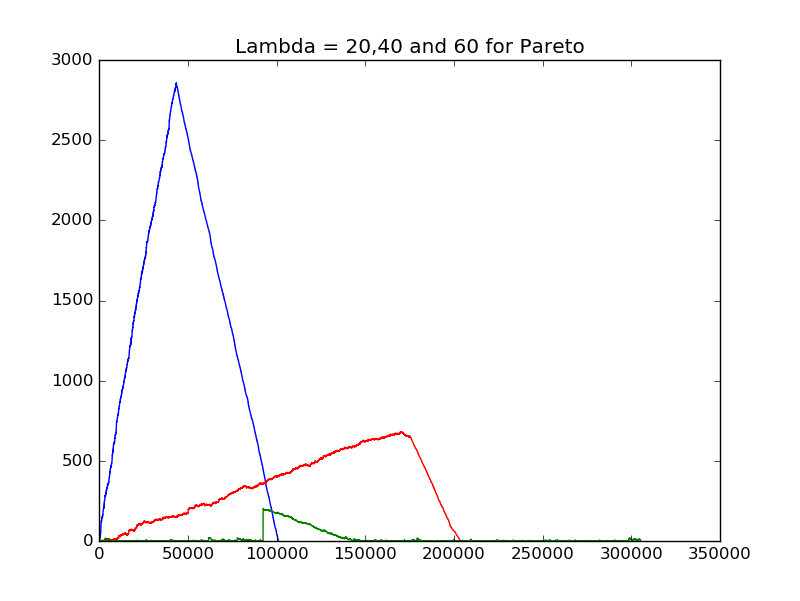
\includegraphics[scale=0.50]{3lambdapareto.png}
\caption{\label{fig:rf_taille_noeud} $\lambda$ = 20,40,60, $users$ = 5000 Pareto}
\end{figure}



\end{document}